\documentclass[a4paper,14pt]{report}

% В этом документе преамбула

%%% Работа с русским языком
\usepackage{cmap}					% поиск в PDF
\usepackage{mathtext} 				% русские буквы в формулах
%\usepackage[T2A]{fontenc}			% кодировка
%\usepackage[utf8]{inputenc}			% кодировка исходного текста
\usepackage[english,russian]{babel}	% локализация и переносы
\usepackage{indentfirst}
\frenchspacing

%%%Шрифты
\usepackage{fontspec}      %% подготавливает загрузку шрифтов Open Type, True Type и др.
\defaultfontfeatures{Ligatures={TeX},Renderer=Basic}  %% свойства шрифтов по умолчанию
\setmainfont[Ligatures={TeX,Historic}]{Times New Roman} %% задаёт основной шрифт документа
\setsansfont{Carlito}                    %% задаёт шрифт без засечек
\setmonofont{Courier New}

\renewcommand{\epsilon}{\ensuremath{\varepsilon}}
\renewcommand{\phi}{\ensuremath{\varphi}}
\renewcommand{\kappa}{\ensuremath{\varkappa}}
\renewcommand{\le}{\ensuremath{\leqslant}}
\renewcommand{\leq}{\ensuremath{\leqslant}}
\renewcommand{\ge}{\ensuremath{\geqslant}}
\renewcommand{\geq}{\ensuremath{\geqslant}}
\renewcommand{\emptyset}{\varnothing}

%%% Дополнительная работа с математикой
\usepackage{amsmath,amsfonts,amssymb,amsthm,mathtools} % AMS
\usepackage{icomma} % "Умная" запятая: $0,2$ --- число, $0, 2$ --- перечисление

%% Номера формул
%\mathtoolsset{showonlyrefs=true} % Показывать номера только у тех формул, на которые есть \eqref{} в тексте.
%\usepackage{leqno} % Нумереация формул слева

%% Свои команды
\DeclareMathOperator{\sgn}{\mathop{sgn}}

%% Перенос знаков в формулах (по Львовскому)
\newcommand*{\hm}[1]{#1\nobreak\discretionary{}
{\hbox{$\mathsurround=0pt #1$}}{}}

%%% Работа с картинками
\usepackage{graphicx}  % Для вставки рисунков
\graphicspath{{images/}{images2/}}  % папки с картинками
\setlength\fboxsep{3pt} % Отступ рамки \fbox{} от рисунка
\setlength\fboxrule{1pt} % Толщина линий рамки \fbox{}
\usepackage{wrapfig} % Обтекание рисунков текстом

%%% Работа с таблицами
\usepackage{array,tabularx,tabulary,booktabs} % Дополнительная работа с таблицами
\usepackage{longtable}  % Длинные таблицы
\usepackage{multirow} % Слияние строк в таблице

%%% Теоремы
\theoremstyle{plain} % Это стиль по умолчанию, его можно не переопределять.
\newtheorem{theorem}{Теорема}[section]
\newtheorem{proposition}[theorem]{Утверждение}
 
\theoremstyle{definition} % "Определение"
\newtheorem{corollary}{Следствие}[theorem]
\newtheorem{problem}{Задача}[section]
 
\theoremstyle{remark} % "Примечание"
\newtheorem*{nonum}{Решение}

%%% Программирование
\usepackage{etoolbox} % логические операторы

%%% Страница
\usepackage{extsizes} % Возможность сделать 14-й шрифт
\usepackage{geometry} % Простой способ задавать поля
	\geometry{top=25mm}
	\geometry{bottom=35mm}
	\geometry{left=35mm}
	\geometry{right=20mm}
 %
%\usepackage{fancyhdr} % Колонтитулы
% 	\pagestyle{fancy}
 	%\renewcommand{\headrulewidth}{0pt}  % Толщина линейки, отчеркивающей верхний колонтитул
% 	\lfoot{Нижний левый}
% 	\rfoot{Нижний правый}
% 	\rhead{Верхний правый}
% 	\chead{Верхний в центре}
% 	\lhead{Верхний левый}
%	\cfoot{Нижний в центре} % По умолчанию здесь номер страницы

\usepackage{setspace} % Интерлиньяж
\onehalfspacing % Интерлиньяж 1.5
%\doublespacing % Интерлиньяж 2
%\singlespacing % Интерлиньяж 1

\usepackage{lastpage} % Узнать, сколько всего страниц в документе.

\usepackage{soul} % Модификаторы начертания

\usepackage{hyperref}
\usepackage[usenames,dvipsnames,svgnames,table,rgb]{xcolor}
\hypersetup{				% Гиперссылки
    unicode=true,           % русские буквы в раздела PDF
    pdftitle={Master's thesis},   % Заголовок
    pdfauthor={Dmitry Velikiy},      % Автор
    pdfsubject={master's thesis},      % Тема
    pdfcreator={Dmitry Velikiy}, % Создатель
    pdfproducer={Dmitry V.}, % Производитель
    pdfkeywords={modelling} {forecast} {social}, % Ключевые слова
    colorlinks=false,       	% false: ссылки в рамках; true: цветные ссылки
    linkcolor=red,          % внутренние ссылки
    citecolor=black,        % на библиографию
    filecolor=magenta,      % на файлы
    urlcolor=cyan           % на URL
}

\usepackage{csquotes} % Еще инструменты для ссылок

%Библиография
\usepackage[backend=biber,bibencoding=utf8,sorting=nty,maxcitenames=4,style=gost-numeric, language=auto, babel=other]{biblatex}
\addbibresource{fuzzy_thesis.bib}

\usepackage{multicol} % Несколько колонок

\usepackage{tikz} % Работа с графикой
\usepackage{pgfplots}
\usepackage{pgfplotstable}
\usepackage{pgfcalendar}

%Счетчик страниц
\usepackage{lastpage}

\author{Дмитрий Великий}
\title{Магистерская диссертация}
\date{\today}

\begin{document} % конец преамбулы, начало документа

\tableofcontents
\chapter*{Введение}
\addcontentsline{toc}{chapter}{Введение}
В современном мире усиливается потребность в автоматизации процессов управления,
в частности административных процессов государственного уровня. Для этого
необходимо создавать информационные системы, отвечающие потребностям лиц,
принимающих решения. Управление социально-экономическим развитием города ---
комплексная задача, включающая в себя управление различными сферами и
подсистемами жизнедеятельности города с целью повышения его экономического,
творческого, научного потенциала, повышения качества жизни горожан, привлечения
инвестиций, создания комфортных условий для предпринимательства, обеспечения
социальной защищённости и благоприятного эмоционально-психологического климата в
городе.

Одним из проблемных явлений в жизни общества является проблема наркомании,
наркотической зависимости. Наркомания наносит ощутимый экономический ущерб
обществу. Но не менее опасен урон общественной морали и принципам благоразумия 
потому, что наркотики разрушительно влияют на мозг человека. А ведь ещё Рене
Декарт провозгласил классический прицип рационализма Нового времени: <<Cogito
ergo sum>>, или <<Мыслю, следовательно существую>>. Таким образом, можно
предположить, что наркотизм причиняет человеку поистине экзистенциальные
страдания. Но несмотря на чисто гуманистические соображения о стремлении помочь
ближнему нужно понимать, что наркотизм --- сложный феномен, полностью победить
который не смогли ещё ни в одной стране мира.

Характерными чертами наркоситуации являются скрытность, обусловленная
её нелегальной природой, сетевой характер распространения, рискованность, но и
прибыльность наркорынка, наличие связей между наркоситуацией и другими
негативными явлениями: безработицей, коррупцией, преступностью и др. Все эти
особенности требуют подходов, которые способны были бы адресовать их.

Общепринятым подходом к организации антинаркотических программ является
использование наукоемкой аналитики для поддержки принятия управленческих решений
ответственными лицами. И здесь большую \textbf{актуальность} имеют модели,
способные не только описать свойства процесса, но и объяснить внутренние
механизмы его протекания, связь наркотизации с другими сферами города,
генерировать т.н.  <<actionable insights>> --- идеи, которые позволяют
действовать: применять конкретные рычаги управления, выявленные при помощи
моделирования, для влияния на наркоситуацию. Более того, интересны модели,
способные к самообучению, универсальной подстройке под исходные данные.

Однако, в практике повседневного информационно-аналитического обеспечения
органов государственной власти в Санкт-Петербурге, в основном, применяются
традиционные модели прогнозирования, известные по эконометрике, математической
статистике: модель авторегрессии с интегрированным скользящим средним, модель
Хольта-Винтерса, модель линейной регрессии и др. Данные модели для своего
корректного применения требуют наложения определённых ограничений на исходные
данные, таких как их линейность, отсутствие т.н. outliers --- случайных
всплесков, наличие сезонных циклов и т.п. В то же время, данные, наблюдаемые при
мониторинге наркоситуации, зачаствую являются нелинейными, неполными,
полученными из экспертных или вовсе неформальных источников. Для учета этих
особенностей могут подходить интеллектуальные методы прогнозрование, одним из
которых является нечеткая логика. Нечеткую логику зачастую применяют вместе с
алгоритмами машинного обучения, такими, как искусственные нейронные сети и др.
Такие авторы, как Н. А. Абдуллавева \cite{Abdullaeva2010}, М. Г. Мамедова, З.Г.
Джабраилова \cite {Mamedova2005}, П. С. Пак, Г. Ким \cite{Pak2005}, А. Сасу
\cite{Sasu2010} демонстрируют, хоть местами и противоречивые, но обнадеживающие
результаты в применении интеллектуальных методов и нечеткой логики для
прогнозирования социальных процессов. 

\textbf{Практическая значимость работы.} Подход к прогнозированию с
использованием методов интеллектуального анализа временных рядов, гипотетически,
может эффективно решить задачу государственного управления и оценки
стратегического развития региона в области борьбы с наркоманией. Для этого
соответствующее программное обеспечение должно быть внедрено в действующие
информационно-аналитические системы. Данныая работаа выполняется по заказу
Санкт-Петербургского информационно-аналитического центра, деятельность которого
связана с разработкой информационно-аналитических систем поддержки принятия
решений в органах государственной власти и местного самоуправления.

\textbf{Цель ВКР} состоит в повышении эффективности поддержки принятия решений
при прогнозировании развития наркоситуации с Санкт-Петербурге. Для достижения
поставленной цели необходимо решить следующие задачи:
\begin{itemize}
\item Обзор существующих в мире политик и моделей организации антинаркотической
деятельности на государственном уровне;
\item Описание используемой в настоящее время системы мониторинга и анализа
наркоситуации в Санкт-Петербурге;
\item Обзор методов и моделей прогнозирования временных рядов;
\item Разработка и опытная проверка метода прогнозирования на основе нечеткой
логики, выработка рекомендаций к применению;
\item Разработка компонента государственной информационной системы, реализующего
новый метод прогнозирования.
\end{itemize}




\chapter{Нечеткое прогнозирование временных рядов}
\newpage
\section*{Введение}
\addcontentsline{toc}{section}{Введение}

Наркоситуация как разновидность социальной ситуации представляет собой 
ограниченную временными и пространственными рамками совокупность социальных 
процессов, складывающихся в результате взаимодействия различных сторон 
общественных отношений.  Рассматривая наркоситуацию как разновидность 
социального взаимодействия, важно в первую очередь использовать системный 
подход, выделяя элементы, составляющие наркоситуацию как систему, а также 
интерпретируя характер взаимодействия между ними.

Полноценное моделирование наркоситуации, по нашему мнению, должно учитывать 
взаимовлияние социально-экономических индикаторов, описывающих наркоситуацию, 
тем самым оно может представлять интуитивно понятную логику протекания 
процессов, и выявлять необходимые для изменения ситуации рычаги управления.  
Немалую роль здесь играет и сам характер доминирующей в стране системы 
управления в области противодействия наркомании.  В данной работе 
рассматривается процесс антинаркотического регулирования <<сверху-вниз>> с тем, 
чтобы согласовать прикладное моделирование с целями, выдвигаемыми государством 
при реализации стратегий развития наркоситуации.

\textbf{Цель работы:} разработка модели прогнозирования доли наркозависимых в 
населении Санкт-Петербурга с помощью индикаторов наркотизации.

\textbf{Поставленные задачи} для достижения цели данной главы:
\begin{itemize}
    \item обзор существующих антинаркотических политик и способов их 
        информационной поддержки.
\end{itemize} 



\newpage
\section{Международный опыт использования информационных систем при реализации 
    государственной антинаркотической политики}

Обеспечение национальной безопасности — одна из важнейших функций государства.  
В Стратегии национальной безопасности Российской Федерации 
\cite{ru_nat_def_strat} наркомания определяется как социально значимое 
заболевание, требующее разработки «единых общероссийских подходов к диагностике, 
лечению и реабилитации пациентов».  Снижение уровня наркомании должно 
способствовать «повышению качества жизни российских граждан».

Однако, существующие модели организации антинаркотической деятельности далеко не 
всегда достигают цели, а бюджетные средства, которые инвестируются в их 
реализацию, не окупаются. Поэтому для исследования актуально обратиться к 
накопленному международному опыту. Предмет данной главы — соотношение между 
антинаркотической политикой государства и информационными системами, призванными 
обеспечить её выполнение. В данной главе приводится обзор основных видов 
наркополитик, обзор и классификация некоторых из существующих в мире 
информационных систем, обеспечивающих противодействие распространению наркомании 
в обществе.

\subsection{Виды антинаркотических политик}

Рассмотрим виды наркополитик. Политика \textbf{снижения потребления} (use 
reduction) нацелена на устранение, или по меньшей мере снижение употребления 
наркотиков в обществе. Уменьшение потребления —  основная цель контроля над 
наркотиками в США, что отражено в Национальной стратегии по борьбе с наркотиками 
(National Drug Control Strategy)\cite{us_nat_drug_strat}. Она также занимает 
видное место в антинаркотических политиках европейских стран, таких как Швеция и 
Франция, а также странах Ближнего Востока. Политика уменьшения потребления 
основывается на мысли, что проблемы, связанные с наркотиками,  возникающие в 
обществе, семье, социальных группах, могут быть решены, только если прекратить 
или минимизировать употребление наркотиков. 

Для людей, которые не употребляют наркотики, парадигма уменьшения потребления 
предполагает профилактические программы, разработанные с намерением 
предотвратить употребление наркотиков.

Политика \textbf{снижения вреда на микроуровне} (micro harm reduction) нацелена 
на снижение среднего вреда отдельным наркозависимым и лицам, не употребляющим 
наркотики. Эта политика опирается на мысль, что само по себе употребление 
наркотиков лишь умеренно опасно, и можно предпринять шаги для уменьшения рисков, 
сопутствующих употреблению наркотиков. Термин «снижение вреда» может 
трактоваться широко, однако эта гибкость может стать источником путаницы, давая 
возможность ввода в действие двух диаметрально противоположных политик, 
направленных при этом одну цель — снижение вреда (например, программы обмена 
шприцев для наркозависимых с целью уменьшения распространения инфекционных 
заболеваний и, следовательно, снижения вреда для наркозависимых, и обязательное 
лишение свободы для лиц, употребляющих наркотики, с целью снижения вреда для 
тех, кто не употребляет). Поэтому при анализе нужно четко определять задачи, 
поскольку есть различные негативные эффекты, связанные с употреблением 
наркотиков, каждый со своим контекстом употребления и противодействия 
наркотикам.

Среди стран, придерживающихся данного подхода, можно выделить Швейцарию, 
Нидерланды, Канаду.
 
Снижение вреда на микроуровне уходит корнями как в общественное здравоохранение, 
так и в более широкое движение за нормализацию употребления наркотиков. 
Внедрение современных методов снижения вреда в населенных пунктах США является 
следствием более ранних европейских опытов с программами обмена шприцев и 
контролируемого распространения наркотиков. 

Мероприятия по реализации антинаркотической политики могут оказывать влияние на 
распространенность, интенсивность и вред от употребления наркотиков. Понятие 
тотального вреда (total harm reduction) охватывает все эти явления. Политика 
\textbf{тотального снижения вреда} объединяет черты снижения потребления и 
снижения вреда на микроуровне \cite{MacCoun2001}. Макровред определяется как 
произведение  распространенности, интенсивности и среднего вреда от наркотиков. 
Тотальный вред определяется как сумма макровредов. Данный подход тесно связан с 
анализом рисков, экономического ущерба и т. д. На данный момент он существует, 
прежде всего, как теоретическая модель. 

С практической точки зрения, можно выстроить антинаркотические мероприятия от 
более строгих (снижение употребления) к менее строгим (снижение вреда): 
полицейский надзор за уличной торговлей наркотиками, полицейские «облавы», 
ограничение оборота прекурсоров, арест за малые нарушения, в т.ч. выращивание 
марихуаны, тестирование на наркотики, вмешательство в частную жизнь 
наркозависимых, их обучение, наркосуды, лечение и реабилитация.

\subsection{Использование информационных систем при реализации антинаркотической 
    политики}

Рассмотрим применение информационных систем при реализации антинаркотической 
политики на примере США, придерживающейся преимущественно политики снижения 
потребления. К категории мониторинговых систем можно отнести PDMP, созданную для 
идентификации лиц, злоупотребляющих наркосодержащими лекарствами, ограничения 
выписывания и продажи данной категории лекарств как государственными, так и 
частными клиниками и аптеками. В эту же категорию входят опросы, такие как ADAM 
(тестирование арестантов на наличие следов приема наркотиков), NSDUH, SAMHDA 
(общенациональные опросы),  National Roadside Survey (тестирование водителей на 
алкоголь и наркотики). 

NADDIS — это система сбора и индексирования данных, содержащая миллионы личных 
дел граждан, для доступа полиции и наркоаналитиков. ADNET — ИС Департамента 
обороны, функции которой — мониторинг, обеспечение мероприятий по снижению 
спроса на наркотики, обеспечение правоприменения как внутри, так и вне страны. 
Проект HIDTA нацелен на координацию деятельности различных государственных 
агентств в т.н. «высокоинтенсивных зонах», в частности на границе с Мексикой, с 
целью пресечения наркотрафика. STRIDE — система извлечения информации о
результатах лабораторного анализа образцов наркотиков из материалов уголовных 
дел по наркопреступлениям.

В Европейском союзе функционирует децентрализованная организация European 
Monitoring Centre for Drugs and Drug Addiction (EMCDDA), которая ежегодно 
публикует отчёты о состоянии наркотических проблем в государствах-членах 
Евросоюза, собирает и предоставляет актуальные эмпирические данные для как для 
учёных, так и для политиков. Деятельность EMCDDA во многом основана на 
информационной сети Reitox, составленной из назначенных национальный институтов, 
ответственных за сбор данных и формирование отчетов по проблемам наркотиков и 
наркомании.  Эти институты носят название <<национальных точек фокуса>> или 
<<национальных пунктов наблюдения за наркоситуацией>>. Эта мониторинговая 
система охватывает 30 стран, причем сбор и обмен данными стандартизирован. В 
Миссии организации указано, что она призвана <<помогать определять направление 
наркополитик Евросоюза, и разрабатывать подходящие рекомендации странам для 
организации лечения, превентивных мер и деятельности по уменьшению вреда>>.

Среди других примеров информационных систем можно привести The Exchange on Drug 
Demand Reduction Action (EDDRA) --- база данных с доступом через Интернет, 
предоставляющая официальным ответственным лицам данные по программам снижения 
спроса на наркотики в Евросоюзе.

В Канаде функционирует Drug Treatment Court Information System, обеспечивающая 
деятельность т.н. <<наркосудов>>, которые являются типичным примером реализации 
политики снижения вреда.

Таким образом, по результатам краткого обзора, обнаруживается, что в странах, 
взявших на вооружение политику снижения употребления, среди ИС превалируют 
мониторинговые системы, отчасти --- аналитические, и на последнем месте --- 
медицинские и ресоциализирующие программы.
С другой стороны, в странах, придерживающихся политики снижения вреда, есть как 
мониторинговые системы, так и и системы, обеспечивающие различные социальные 
программы по снижению вреда.

\subsection{Зарубежный опыт прогнозирования распространения наркомании}

Рассмотрим подходы к прогнозированию наркоситуации с использованием эмпирических
данных (социологических опросов и др.) в странах Евросоюза и США.

В монографии центра EMCDDA дается обзор методов моделирования т.н. <<потребления
наркотиков с высокой степенью риска>> (high-risk drug use) или <<проблемного
употребления наркотиков>> (problem drug use) в Европе \cite{EMCDDA2001}. Описан
метод прогнозирования распространения наркомании с использованием ГИС
\cite{EMCDDA2001,Wiessing1999}, разработанный в рамках программы DIPEP --- Drug
Incidence \& Prevalence Estimation Program. Распространение наркомании
моделируется как процесс, схожий с заражением в эпидемиологии. В этой парадигме
ключевыми понятиями являются пути передачи инфекции, группы риска,
распространенность инфекции, её географическое распределение, эпидемический
цикл. Зоны распространения наркомании моделируются с помощью метода обратных
взвешенных расстояний. Таким образом моделируется изменение частоты и
распространенности потребления наркотиков в Великобритании.  На примере города
Глазгоу показана первоначальная концентрация <<наркоэпидемии>> внутри крупного
города с последующим распространением в окрестные города в течение пятилетних
циклов. 

Для оценки численности наркозависимых предлагается применение множества
динамических моделей, использующих доступные статистические данные. В данном
подходе основополагающим тезисом является необходимость уменьшить
неопределенность, связанную со скрытым характером процессов, характеризующих
наркоситуацию. Для этого применяются методы стратифицированных калибровочных
выборок, вероятностное моделирование, процессы Пуассона, метод множественного
захвата и перезахвата, оценка по связи распространенности тяжелых наркотиков и
частоте аквизитивных преступлений, марковские модели. Применение множества
методов и моделей для оценки одной целевой популяции позволяет более точно
судить о трендах и о порядке численности наркозависимых. 

В качестве альтернативной модели прогнозирования наркоситуации предлагается
модель с множеством индикаторов. В данной модели строится гипотеза о
существовании связей типа <<причина-следствие>> между индикаторами. Выделяется
три группы индикаторов: 
\begin{itemize}
    \item социальные;
    \item правовые;
    \item медицинские.
\end{itemize}
Авторами отмечается универсальность данной модели, возможность её использования
для исследования различных социально-экономических сценариев, адаптация модели к
исходным данным. Практическое применение данной модели позволило получить
неожиданные и контринтуитивные результаты. 

Отдельно европейскими исследователями выделяется класс динамических моделей.
Термин <<динамическая модель>> охватывает методы системного анализа и
моделирования временных рядов, применяемые для оценки распространенности
наркопотребления. Данные методы должны обеспечивать не только дескриптивный
анализ, но и моделировать процессы, лежащие в основе наркоситуации. Динамические
модели в отличие от статических описывают процессы во времени. Например,
исследуемым процессом может быть изменение состояния наркопотребителей в модели
<<поимка-мечение-повторная поимка>>. Модели поимки-повторной поимки делятся на
два класса: с открытой популяцией и с закрытой популяцией. В моделях с закрытой
популяцией предполагается, что популяция не изменяется на протяжении
исследуемого периода, а в моделях с открытой популяцией учитывается прибыль и
убыль особей популяции. Модели с закрытой популяцией проще и предназначены
скорее для анализа коротких временных периодов, но при достаточно большом
временном отрезке они, как правило, необъективны, и в таких случаях применяются
блее сложные модели с открытой популяцией.

В США прогнозирование осуществляется...

В отчете Национального Института правосудия США \cite{TravisFeucht1995, Chaiken1993}
приводится анализ наркоситуации в 23 крупнейших городах США. Датасет состоит из
данных уриноанализа (на предмет позитивного тестирования на кокаин, марихуану,
опиаты) арестантов в разрезе по типам преступлений. Эта информация, в частности,
была использована для установления и объяснения связи между наркотиками и
преступностью. На основании снижения частоты позитивных тестов на кокаин среди
мужчин 15-20 лет строится гипотеза о продолжительном снижении употребления
кокаина по мере того, как представители данной возрастной группы стареют.

В работе Дж. Колкинса \cite{Caulkins1995} производится оценка эластичности спроса 
на кокаин и героин на основании датасетов DUF и STRIDE, предоставленных
Национальным институтом правосудия США и Управлением по борьбе с наркотиками.
Автор пытается ответить на вопрос: насколько изменится потребление при
увеличении цен? В качестве метода математического анализа использованы
дифференциальные уравнения. Анализ показывает высокую эластичность спроса. В
качестве выводов автор связывает подъем употребления кокаина и героина в 1980-х
с существенным снижением цен на них. Как следствие, для проведения
антинаркотической политики могуть быть полезными мероприятия, приводящие к
повышению цен на наркотики.

Датасеты ADAM и ADAM II Trens annualizing statistics\cite{Hunt2013}


\newpage
\section*{Выводы по главе 1}
\addcontentsline{toc}{section}{Выводы по главе 1}

В главе был проведен обзор видов наркополитик, в общем виде описывающих 
концептуальные основы и практические меры по урегулированию наркоситуации.  
Исследована связь между постулируемыми в странах стратегиями антинаркотической 
политики и средствами её информационной поддержки.


\chapter{Опыты нечеткого прогнозирования}
\newpage
\section*{Введение}
\addcontentsline{toc}{section}{Введение}

Цель данной главы – анализ применимости новых моделей прогнозирования к задачам государственного управления.

Для достижения указанной цели необходимо решить следующие задачи:
\begin{enumerate}
    \item обзор литературы по теме прогнозирования временных рядов, и в особенности, интеллектуального прогнозирования
    \item выявление сфер применения новых методов прогнозирования, степени их теоретической проработки и практических результатов их использования.    
    \item обзор программных пакетов, позволяющих реализовывать методы нечеткого прогнозирования.
\end{enumerate}
Работа выполняется по заказу Санкт-Петербургского информационно-аналитического центра.

\newpage
\section{Задачи прогнозирования и интеллектуальный анализ временных рядов}

Количество информации, порождаемой человечеством, непрерывно растет \cite{Gantz2011}. 
В связи с этим все важнее становится умение анализировать данные, извлекать из них знания, чтобы превратить в движущую силу социально-экономического развития. 

Одним из методов анализа данных является прогнозирование. 
Прогнозная аналитика использует методы математического моделирования, искусственного интеллекта и теории игр, 
анализирует текущие и исторические факты для составления предсказаний о будущих событиях. 
Фиксируются связи между разными факторами, на основании их выявления идентифицируются риски и возможности. 
Задача прогнозирования лежит в основе финансового планирования в экономике, управления объемами производства, принятия решений в сфере управления социальными системами.

На сегодняшний день существует множество моделей прогнозирования временных рядов \cite{Chuchueva2012}: регрессионные и авторегрессионные, 
нейросетевые, экспоненциального сглаживания, на базе цепей Маркова, классификационные и др. (Рис. ~\ref{figure:mod_classifier}).
\begin{figure}[bhtp]
    \centering
    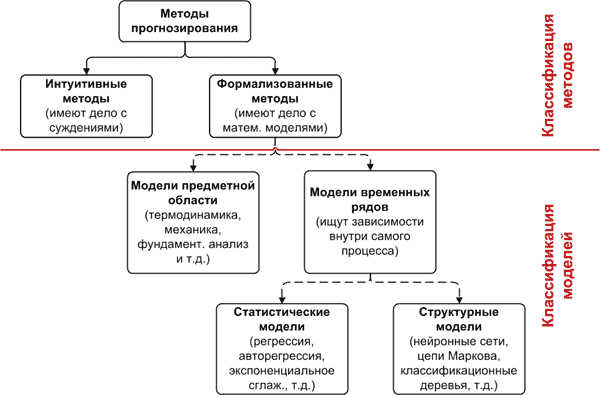
\includegraphics[width=\textwidth, keepaspectratio]{images/mod_classifier.png}
    \caption{классификация моделей и методов прогнозирования \cite{Chuchueva13habr}}
    \label{figure:mod_classifier}
\end{figure}
Прогнозирование в государственном управлении осуществляется посредством разных методов: экстраполяции, факторного прогнозирования, 
модельного прогнозирования, экспертного оценивания. 
Органы государственной власти в последние годы все чаще обращаются к методу экспертного прогнозирования \cite{Gegedush2008}. 
В этом случае эксперт дает прогноз, опираясь на опыт, аналогии, интуицию. 
В то же время интуитивная природа данного метода заставляет при его использовании полагаться лишь на квалификацию и репутацию эксперта, 
тем самым внося дополнительную неопределенность в процесс прогнозирования. 
Существуют исследования, показывающие, что прогнозы экспертов по точности уступают прогнозам на основе моделирования. 
П. Мийл на примере 20 прогнозов из области клинической диагностики \cite{MeehlClinStat} 
и Дж. Сойер на примере 45 прогнозов в социальной сфере \cite{Sawyer1966} демонстрируют тот факт, 
что экспертные оценки ни в одном из перечисленных случаев не были существенно точнее статистических моделей прогнозирования. 
Кроме того, наблюдается нехватка специалистов по работе с данными \cite{Davenport2012}. 
Все это побуждает задуматься о других подходах к анализу данных. 

В последние два десятилетия активно развивается направление прогнозирования, связанное с интеллектуальным анализом временных рядов \cite{Yarushkina2010}. 
Основными целями этого направления являются, во-первых, анализ и моделирование процессов, характеризующихся высокой степенью неопределенности, 
в том числе в областях, слабо подверженных формализации, 
во-вторых, повышение уровня интеллектуальной поддержки современных специалистов, 
и, в-третьих, выявление скрытых закономерностей и извлечение новых знаний из временных рядов. 

\newpage
\section{Сферы применения методов интеллектуального анализа временных рядов}

В основе новых методов анализа временных рядов лежит нечеткая модель временного ряда. 
Теория нечетких множеств была впервые изложена Л. Заде в 1965 г. \cite{zadeh1965fuzzy}. 
В 1973 г. предложена теория нечеткой логики \cite{Zadeh1973}. 
Вскоре после этого теория стала популярна. 
В конце 1980-х гг. это направление стало бурно развиваться в Японии. 
Нечеткое управление стало применяться в промышленности, железнодорожном транспорте и разработке потребительской техники.

\begin{figure}[h]
    \centering
    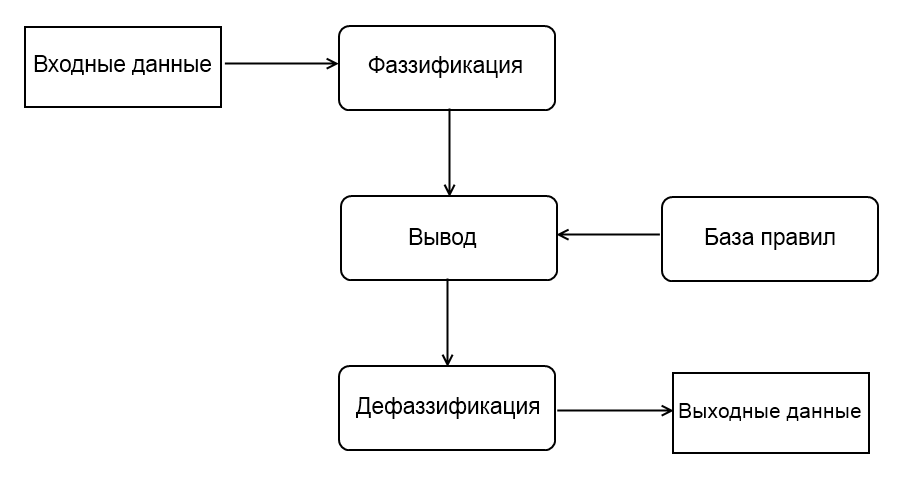
\includegraphics[width=\textwidth, keepaspectratio]{images/fuzzy_engine.png}
    \caption{Система нечеткого вывода}
    \label{figure:fuzzy_engine}
\end{figure}

Основной идеей нечеткой логики является многозначность. 
Высказывание может иметь любое истинностное значение в промежутке от 0 до 1. 
Таким образом, воспроизводится неточность человеческого мышления.

Модели статических и динамических систем, построение, 
использование и анализ которых базируется на положениях теории нечетких множеств и нечеткой логики, называют нечеткими моделями или нечеткими системами. 
Целью нечеткого моделирования сложных явлений является приближенное описание зависимости. 

В основе нечетких продукционных моделей лежит совокупность нечетких правил «ЕСЛИ, ТО», 
описывающих зависимости между нечеткими переменными предметной области, 
композиционное правило вывода и способ вычисления значений нечетких переменных (способ нечеткого вывода).

Модель описания поведения систем на естественном (или близком к естественному) языке,
в виде приближенных рассуждений в теории нечетких множеств и нечеткой логики,
основанная на композиционном правиле вывода, называется системой нечеткого логического вывода.

В систему нечеткого логического вывода входят следующие объекты (рис. ~\ref{figure:fuzzy_engine}):
\begin{enumerate} 
    \item совокупность нечетких продукционных правил (база правил);
    \item блок фаззификации;
    \item блок дефаззификации;
    \item блок вывода.
\end{enumerate}

На основании общей модели, приведенной выше, создаются контроллеры для управления преимущественно техническими объектами.

В начале 1990-х гг. была предложена теория нечетких временных рядов \cite{Song1993}. 
Нечетким временным рядом называют упорядоченную в равноотстоящие моменты времени последовательность наблюдений над некоторым процессом,
состояния которого изменяются во времени, если значение состояния процесса в данный момент времени может быть выражено с помощью нечеткой метки. 
Нечеткая метка может быть сформирована непосредственно экспертом или получена на основе некоторого преобразования исходного временного ряда \cite{Yarushkina2010}. 

В условиях, когда моделируемым процессам присуща высокая степень неопределенности, 
методы прогнозирования на основе нечетких моделей временных рядов позволяют выработать наиболее адекватную оценку будущих изменений в социально-экономических системах.

Ряд исследований \cite{Chen1996,S.Melike2008,Saxena2012}, в которых изучается прогнозирование с помощью моделей нечетких временный рядов, 
демонстрирует положительные результаты. 
Точность прогнозирования улучшается за счет использования генетических алгоритмов для настройки параметров нечетких моделей прогнозирования, 
изменения количества нечетких множеств, используемых для описания временного ряда, использование достаточного числа продукционных правил, 
модификации интервалов, на которые разбивается исходный ряд и др.

В то же время есть примеры неудовлетворительного применения нечеткой логики в прогнозировании временных рядов \cite{Hoekstr2010}. 
Причиной тому неопределенность при создании набора продукционных правил, необходимость адекватного выбора переменных, 
включаемых в модель, сложность построения модели ввиду новизны, малой изученности данной темы и большой вариативности при построении модели.

\newpage
\section{Программные средства интеллектуального прогнозирования}

Для использования прогнозирования в принятии решений целесообразным может оказаться интеграция этих моделей с экспертной системой или системой поддержки принятия решений. 
В этом случае нужно задуматься о программной реализации нечетко-логических моделей. 
Попробуем рассмотреть существующие библиотеки, в той или иной мере охватывающие тему нечеткой логики, нечеткого вывода и т.д.

\textit{Fuzzy Logic Toolbox для Matlab}. Хотя данный продукт имеет все необходимые возможности, для наших задач он не подходит, т.к. функционирует на собственном языке программирования и является платным.

\textit{Fuzzy Logic Toolkit для Octave.} Аналог Fuzzy Logic Toolbox, относящийся к категории программного обеспечения с открытым исходным кодом. Распространяется по лицензии GPLv2, ограничивающей его использование в коммерческой деятельности.

\textit{jFuzzyLogic}. Позиционируется как наиболее полная библиотека по нечеткой логике и стандарт де-факто в исследовательской и прикладной деятельности. Тем не менее, обладает таким недостатком как сложность в использовании.

\textit{jfuzzylite.} Еще одна альтернатива, отличительными чертами которой являются открытый исходный код, наиболее свободная лицензия, простота в использовании, наличие различных алгоритмов вывода, лингвистических переменных, операторов нечеткой логики. Также планируются дополнения в виде новых нечетких контроллеров, алгоритмов кластеризации и адаптивных нейро-нечетких систем вывода.

\textit{FuzzyEngine, funzy и др.} либо неполны, либо заточены под чисто учебные цели и поэтому непригодны для наших задач. 

По итогам обзора можно выделить jfuzzylite и jFuzzyLogic в качестве основных претендентов к использованию.

\newpage
\section*{Выводы по главе 2}
\addcontentsline{toc}{section}{Выводы по главе 2}

На основе обзора методов прогнозирования, анализа динамики применения этих методов в прошедшие десятилетия, 
обзора программных библиотек, реализующих принципы нечеткой логики, сделаны следующие выводы:
\begin{enumerate}
    \item Увеличение размерности и доли неопределенности в наблюдаемых данных приводят к необходимости искать новые методы анализа и прогнозирования данных.
    \item Интеллектуальные методы анализа данных дают противоречивые результаты в силу малой изученности и проблемности данной области. Тем не менее, наблюдается положительная тенденция в сторону уточнения моделей.
    \item Существующие свободно распространяемые программные библиотеки позволяют реализовывать системы нечеткого вывода. 
\end{enumerate}

Рассматриваемые нечеткие модели прогнозирования временных рядов, помимо ликвидации неопределенности и возможности работать со слабо формализуемыми входными данными, 
обладают преимуществом простоты для пользователя благодаря использованию продукционной модели знаний. 
Данная модель оперирует правилами, написанными естественным языком, что позволяет пользоваться и совершенствовать её специалисту в предметной области, 
а не только разработчику метода и программной реализации прогнозирования. 
Это положительно сказывается на адекватности прогноза.

Выбранный подход к прогнозированию с использованием методов интеллектуального анализа временных рядов и нечеткой логики имеет потенциал для того, 
чтобы эффективно решить задачу государственного управления и оценки стратегического развития региона. 
Для этого соответствующее программное обеспечение должно быть внедрено в действующие информационно-аналитические системы. 

Дальнейшая работа будет связана с адаптацией какой-либо нечеткой модели 
и её программной реализацией для опытного оценивания возможностей интеллектуального анализа временных рядов.



\chapter{Разработка модели прогнозирования численности наркозависимых в 
Санкт-Петербурге на основе нечеткой модели с многими переменными}
\section*{Введение}
\addcontentsline{toc}{section}{Введение}

Проблема эффективного прогнозирования социально-экономических процессов в настоящее является исключительно актуальной задачей. Особенную сложность прогнозирование приобретает в задачах государственного управления. В силу того, что государственные планы и прогнозы затрагивают жизнь большого числа людей, возрастает цена ошибки. Поэтому необходимо минимизировать риски. Одним из способов минимизации рисков является научный подход в прогнозировании возможных сценариев развития общества.  

Социально-экономическим процессам свойственны неопределенность, наличие скрытых факторов влияния, слабая предсказуемость. Системы, характеризующиеся такими процессами, называют нелинейными, хаотическими, случайными, неопределенными. Существуют математические теории, призванные <<уточнять>> неточности: теория детерминированного хаоса, теория вероятностей, нечеткая логика и др. В данной работе рассматриваются прикладные аспекты социального прогнозирования с помощью нечеткой логики.

\textbf{Цель данной главы:} разработка модели прогнозирования доли
наркозависимых в населении Санкт-Петербурга с помощью индикаторов
наркотизации.%выяснение перспектив применения одномерных нечетких моделей.

\textbf{Поставленные задачи} для достижения цели главы:
\begin{itemize}
    \item опытная проверка результатов одномерных нечетко-логических моделей и
        сравнение с	моделями на основе теории нечетких временных рядов.
    \item опытная оценка результатов многомерных нечетко-логических моделей, 
        задействующих в качестве предикторов социально-экономические показатели.
\end{itemize} 

\section{Вычислительный эксперимент нечеткой авторегрессии}

\subsection{Используемые программные средства}

В настоящей статье программная реализация методов нечеткого прогнозирования
базируется на библиотеке <<frbs>> языка статистического программирования R. Библиотека разработана докторами философии и аспирантами Гранадского университета. В библиотеке реализовано более 15 методов нечеткой классификации и регрессии. В библиотеке рассматриваются системы с многими входами и единым выходом (MISO) с данными в виде вещественных чисел.

СНВ --- система нечеткого вывода.
\begin{enumerate}
\item СНВ, основанные на разбиении области определения.
\begin{itemize}
\item Метод Ванга и Менделя. Предназначен для решения задач регрессии \cite{Wang1992}.
\item Метод Чи. Предназначен для решения задач классификации \cite{Chi1996}.
\item Взвешенный метод Ишибучи. Предназначен для решения задач классификации \cite{Ishibuchi2001}.
\end{itemize}
\item СНВ, основанные на искусственных нейронных сетях.
\begin{itemize}
	\item Адаптивная нечеткая система вывода с использованием нейросети. Предназначена для решения задач регрессии \cite{Jan1993}. 
	\item Гибридная нечеткая система вывода с использованием нейросети.  Предназначена для решения задач регрессии \cite{Kim1999}.
\end{itemize}
\item СНВ, основанные на алгоритмах кластеризации.
\begin{itemize}
	\item Субтрактивная кластеризация и метод нечеткой кластеризации c-средних.
	Предназначена для решения задач регрессии \cite{Chiu1996}.
	\item Динамическая эволюционирующая система вывода с использованием нейросети. Предназначена для решения задач регрессии \cite{Kasabov2002}.
\end{itemize}	
\item СНВ, основанные на генетических алгоритмах.
\begin{itemize}
	\item Метод Трифта. Предназначен для решения задач регрессии \cite{Thrift1991}.
	\item Генетическая нечеткая система для обучения нечетких правил, основанная на технологии MOGUL. Предназначен для решения задач регрессии \cite{Cordon1999}.
	\item Метод Ишибучи, основанный на генетическом кооперативно-кон\-курентном обучении. Предназначен для решения задач классификации \cite{Ishibuchi1999}.
	\item Метод Ишибучи, основанный на гибридизации генетического ко\-оперативно-конкурентного обучения и Питтсбургского метода. 
	 Предназначен для решения задач классификации \cite{Ishibuchi2005}.
	\item Структурный обучающий алгоритм на нечеткой среде.  
	Предназначен для решения задач классификации \cite{Gonzalez2001}. 
	\item Генетический алгоритм для латеральной настройки и выбора правил лингвистической нечеткой системы. 
	Предназначен для решения задач регрессии \cite{Alcala2007}.
\end{itemize}
\item СНВ, основанные на методе градиентного спуска.
\begin{itemize}
	\item СНВ с использованием эвристик и градиентного спуска. Предназначена для решения задач регрессии \cite{Ishibuchi1994}.
	\item Правила нечеткого вывода по методу спуска. 
	Предназначен для решения задач регрессии \cite{Nomura1992}. 
\end{itemize}
\end{enumerate}

\subsection{Методика проведения эксперимента}

Основными направлениями нечеткого прогнозного моделирования, описанными в литературе, являются теория нечеткой логики \cite{Zadeh1973} и теория нечетких временных рядов \cite{Song1993}.
При этом, для прогнозирования по методу нечетких временных рядов исследователям удалось добиться существенного снижения погрешности прогнозов даже для авторегрессионного случая. 

Известно \cite{sep-principia-mathematica}, что до некоторых пределов математика сводима к логике. Это и будет исходной точкой нашего эксперимента. Попробуем сравнить доказанные в своей успешности методы теории нечетких временных рядов (основанные на математической теории нечетких множеств) с методами нечеткой логики, реализованными в пакете <<frbs>>.  

Объектом прогнозирования являются данные по поступившим в университет Алабамы абитуриентам за период 1971-1992 гг. (см. Рис.~\ref{figure:UA_enrollments}). Именно они были использованы в статье, впервые описавшей теорию нечетких временных рядов и с тех пор являются основой для сравнения моделей.  

\begin{figure}[bhtp]
	\begin{center}			
		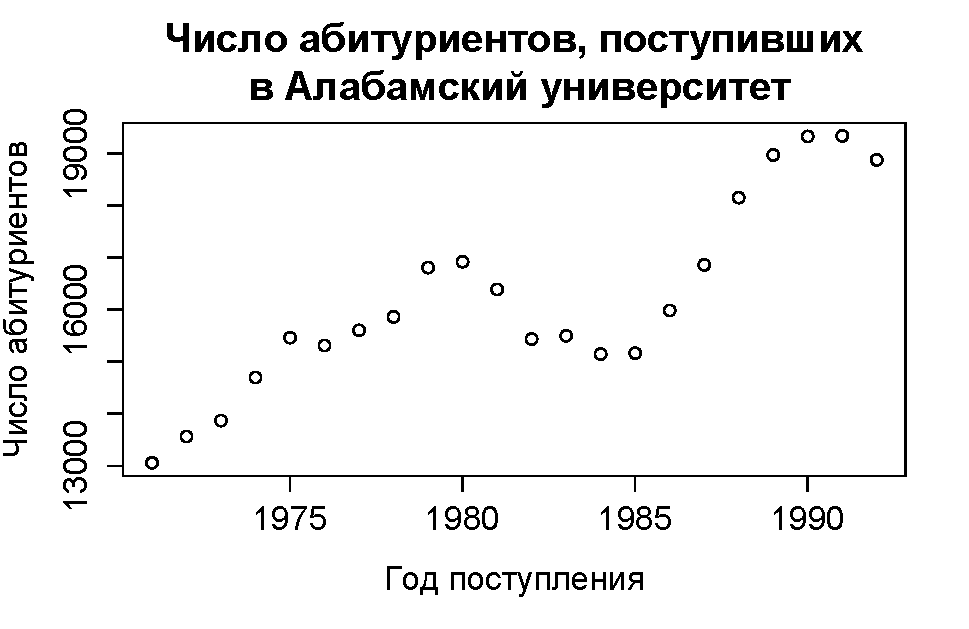
\includegraphics{images/UA_enrollments.pdf}
		\caption{Число поступивших в Алабамский университет, 1971-1992.}		
		\label{figure:UA_enrollments}
	\end{center}
\end{figure}

По итогам экспресс-теста регрессионных моделей решено было выбрать модель авторов Л-Х. Ванга и Дж. М. Менделя, основанную на разбиении области определения \cite{Wang1992}. Критериями отбора были точность прогноза на тестовых данных и сложность вычислений. Модель демонстрирует хорошую точность и низкую вычислительную сложность. 

Алгоритм Ванга и Менделя состоит из пяти шагов:
\begin{enumerate}
	\item Разбиение областей определения входных и выходных численных данных на нечеткие интервалы.
	\item Генерация нечетких правил на основе предоставленных данных.
	\item Присвоение степени каждому из сгенерированных правил с целью разрешения противоречий между правилами.
	\item Создание комбинированной нечеткой базы правил, основанной одновременно на 1) автоматически сгенерированных правилах и
	   2) правилах на естественном языке, предложенных экспертами.
	
	\item Определение отображения входного пространства на выходное, основываясь на комбинированной базе правил, с помощью процедуры дефаззификации.
\end{enumerate}

Доказана возможность предлагаемого отображения аппроксимировать любую непрерывную функцию вещественного переменного на компактном множестве с произвольной точностью.
Примеры нечетких правил и функций принадлежности, генерируемых моделью, см. на
Табл.~\ref{table:fuzzy_rules_example} и Рис.~\ref{figure:MFexample}, соответственно.  

\renewcommand{\arraystretch}{1.5} %Space between rows
\setlength{\tabcolsep}{8pt} %Space between columns

\begin{table}[bhtp]
	\caption{Пример нечетких правил.}
	\begin{center}
		\begin{tabular}{ | c | c | }
			\hline
			1 & IF tminus2 is  v.1\_a.1 and tminus1 is  v.2\_a.1 THEN   t  is  c.1 \\
			\hline
			2 & IF tminus2 is  v.1\_a.7 and tminus1 is  v.2\_a.7 THEN   t  is  c.5  \\
			\hline
			\multicolumn{2}{ |c| }{\ldots} \\
			\hline
			17 & IF tminus2 is  v.1\_a.9 and tminus1 is  v.2\_a.6 THEN   t  is  c.7 \\
			\hline
		\end{tabular}		
	\end{center}
	\label{table:fuzzy_rules_example}	
\end{table}

\begin{figure}[bhtp]
	\begin{center}
		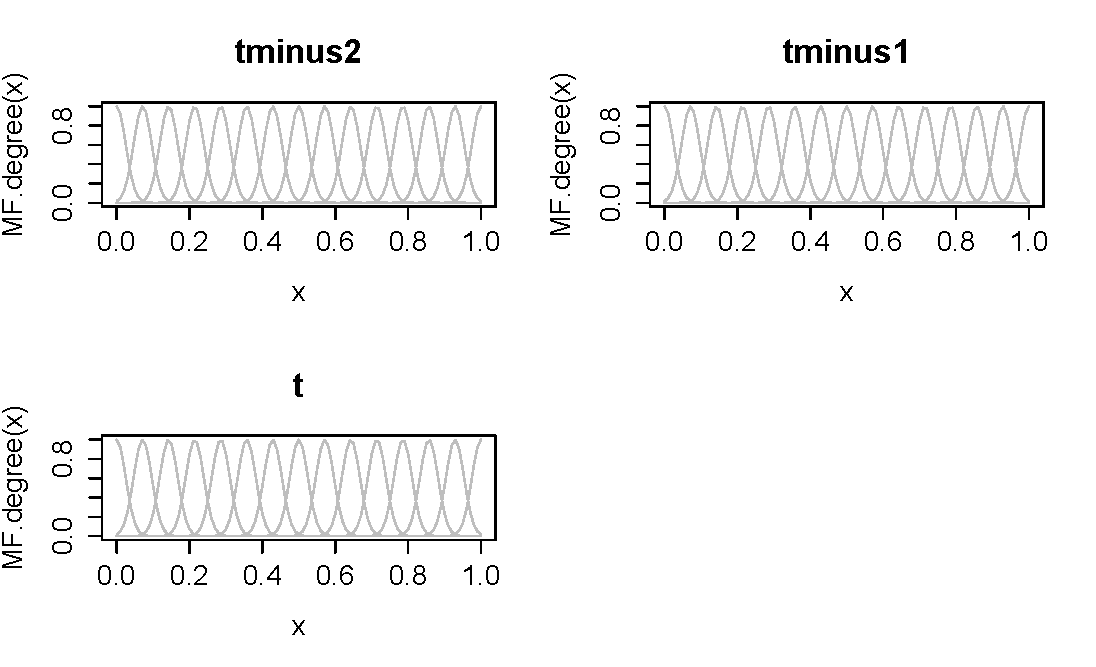
\includegraphics[scale=0.8]{images/MFexample.pdf}
		\caption{Пример функций принадлежности для лингвистических переменных.}		
		\label{figure:MFexample}
	\end{center}
\end{figure}

На выходе модели --- численность поступивших в университет Алабамы за период 1971-1992 гг. ($t$). На входе --- эта же переменная, но со сдвигом на один ($tminus1$) и два ($tminus2$) года назад, соответственно. Таким образом реализована импровизированная авторегрессия по переменной $t$. 

Аналогичным образом в тестовых примерах библиотеки <<frbs>> прогнозировались хаотические временные ряды Маки-Гласса, при этом, однако, сдвиг происходил на 4 и 8 позиций назад и общее число наблюдений составляло 300, а не 22, как в случае с временным рядом поступивших в университет Алабамы.

Общее множество данных разбивалось на два подмножества --- данные для обучения модели и данные для сравнения результатов работы модели --- в зависимости от величины горизонта прогнозирования. 

\subsection{Результаты эксперимента}

В эксперименте использовались два значения горизонта прогнозирования --- 5 лет (см. Рис.~\ref{figure:UA_model_h=5}) и 3 года (см. Рис.~\ref{figure:UA_model_h=3}). Заметим, что в обоих случаях симуляция в области данных для обучения сработала достаточно хорошо, несмотря на крайне малый объем выборки. 

\begin{figure}[bhtp]
	\begin{center}
		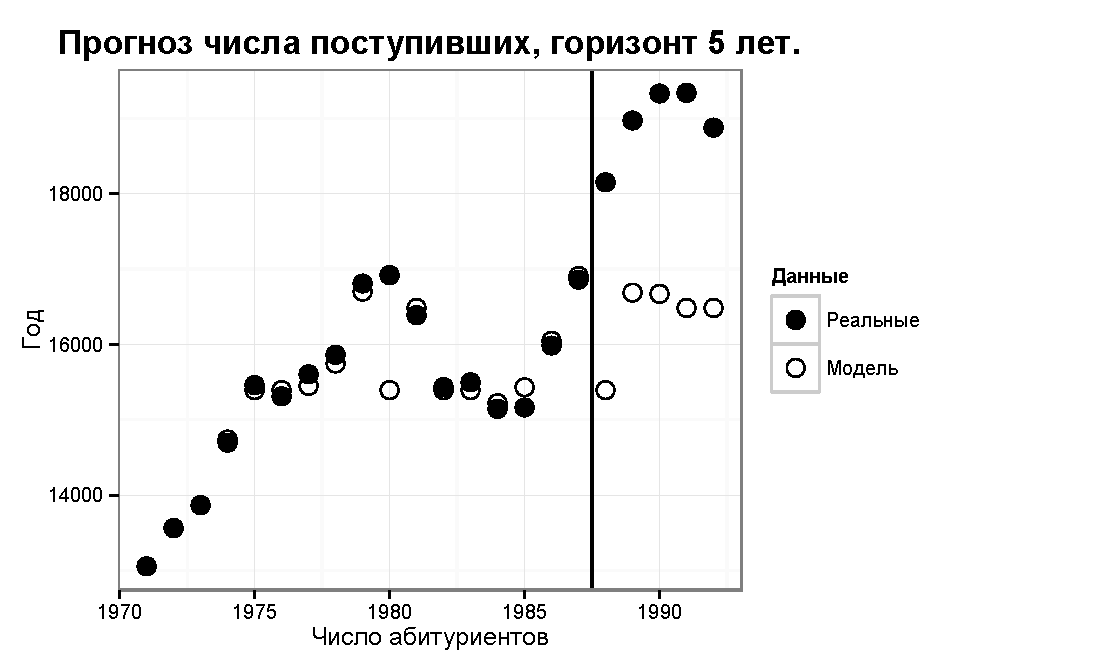
\includegraphics{images/UA_model_h=5.pdf}
		\caption{Прогноз числа поступивших в Алабамский университет, \newline горизонт 5 лет.}		
		\label{figure:UA_model_h=5}
	\end{center}
\end{figure}

\begin{figure}[bhtp]
	\begin{center}
		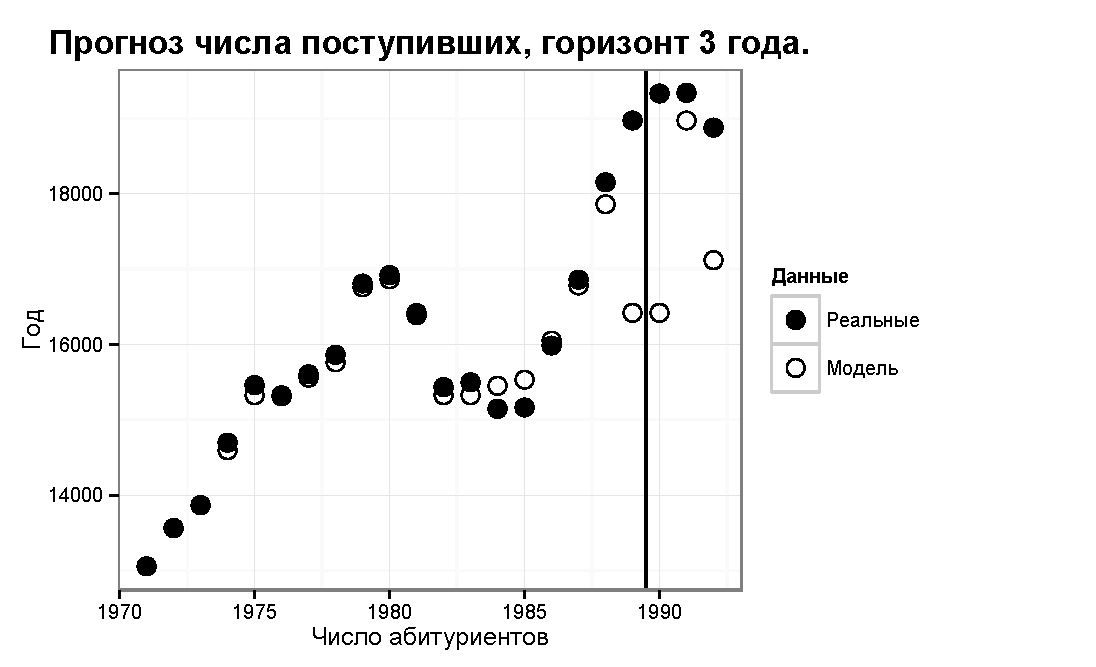
\includegraphics{images/UA_model_h=3.pdf}
		\caption{Прогноз числа поступивших в Алабамский университет, \newline горизонт 3 года.}		
		\label{figure:UA_model_h=3}
	\end{center}
\end{figure}

В части прогноза же результаты неудовлетворительные. Это подтверждается и оценкой погрешности прогнозирования (см. Табл.~\ref{table:WM-error}). Погрешность гораздо выше, чем при авторегрессии методами нечетких временных рядов. С другой стороны, точность увеличивается при уменьшении горизонта прогнозирования. Это говорит о том, что модель адаптируется при изменении параметров и входных данных. 

\begin{table}[bhtp]
	\caption{Оценка точности результатов прогнозирования.}
	\begin{center}
		\begin{tabular}{ | c | c | c | c | }
			\hline
			Горизонт & MSE & RMSE & SMAPE \\
			\hline
			5 & 6.750612e+06 & 2.598194e+03 & 3.674307e+00  \\
			\hline
			3 & 3.897863e+06 & 1.974301e+03 & 2.330708e+00  \\
			\hline
		\end{tabular}		
	\end{center}
	\label{table:WM-error}	
\end{table}

Основной причиной низкой точности прогноза, по нашему предположению, является недостаточность исходных данных. Расширение доступной для модели информации с целью повышения качества прогноза может происходить по трем направлениям:
\begin{itemize}
	\item Увеличение объема выборки (периода, который охватывает временной ряд).
	\item Увеличение количества продукционных правил либо изменение существующих правил.
	\item Увеличение количества либо изменение структуры входных показателей, отбор наиболее релевантных задаче показателей.
\end{itemize}

В процессе вычислительного эксперимента автор столкнулся с техническими трудностями:
\begin{itemize}
	\item Невозможность оценки всех моделей из библиотеки <<frbs>> с варьированием всех параметров моделей ввиду нехватки вычислительных мощностей.
	\item Сложность доступа к данным.  
\end{itemize}
	

\section{Разработка модели прогнозирования численности наркозависимых в 
    Санкт-Петербурге на основе нечеткой модели с многими переменными}

В связи с расширением масштабов незаконного оборота и немедицинского потребления 
наркотиков  в России и в ответ на усиление таких негативных тенденций, связанных 
с наркоситуацией, как устойчивое сокращение численности населения России, в том 
числе уменьшение численности молодого трудоспособного населения, была принята 
Стратегия государственной антинаркотической политики
Российской Федерации до 2020 года \cite{ru_nat_drug_strat}. 

В качестве генеральной цели Стратегии постулируется <<существенное сокращение 
незаконного распространения и немедицинского потребления наркотиков>>. Таким 
образом, можно утверждать, что Российская Федерации придерживается 
преимущественно политики снижения потребления. Это и будет предпосылкой к 
дальнейшим положениям.

\subsection{Теоретико-методологические основы анализа наркоситуации}

По мнению теоретиков анализа наркоситуации \cite{Karpets2010}, с позиций
социального управления приобщение части населения к употреблению психоактивных
веществ целесообразно рассматривать как риск. С точки зрения управления, риск
–-- это событие или группа однородных случайных событий, которому присущи два
основных свойства --– вероятность и ущерб.

Вероятность –-- признак, означающий возможность с той или иной степенью точности
рассчитать и прогнозировать частоту наступления неблагоприятного события (в
данном случае --– акта потребления наркотиков) при наличии достаточного
количества данных и результатов наблюдений. Вместе с тем для риска всегда
характерна случайность, непредсказуемость наступления события, означающая
невозможность точно определить время и место его возникновения. А поскольку риск
выбора потребления наркотиков в современном российском обществе сохраняется, то,
с позиций социального управления, управление антинаркотической деятельностью, а
через него –-- и организация влияния на наркоситуацию и контроля за
проявляющимися в ее рамках тенденциями –-- это прежде всего управление рисками.

Одним из важнейших вопросов исследования наркоситуации выступает анализ и
оценка факторов риска, прямо или косвенно влияющих на тенденции наркотизации. 
Факторы риска можно разделить на две группы:
\begin{enumerate}
    \item факторы, имманентно присущие субъекту наркотизации:
        \begin{itemize}
            \item наследственные
            \item гендер
            \item возраст
            \item социальный статус
            \item социокультурные факторы
        \end{itemize}
    \item внешние факторы:
        \begin{itemize}
            \item доступность наркотических и иных психоактивных веществ
            \item информационные факторы	
        \end{itemize}
\end{enumerate}	

Помимо непосредственно факторов наркотизации для анализа 
целесообразно рассмотреть \textbf{индикаторы воздействия}, т.е. статистические 
и эпидемиологические показатели, отражающие криминальную ситуацию, социальное 
положение и состояние здоровья населения.  Основными индикаторами воздействия 
определены следующие:
\begin{enumerate}		
    \item Социально-демографические и экономические:
    \begin{itemize}
        \item число и доля лиц, попробовавших наркотики хотя бы раз в жизни;
        \item процент лиц определенной возрастной группы, употребляющих наркотики;
        \item спрос на наркотики среди населения;
        \item спектр употребляемых наркотиков;
        \item средняя продолжительность и качество жизни населения;
        \item сумма социально-экономического ущерба от наркотиков (социальная 
            стоимость употребления наркотиков).
    \end{itemize}
    \item Медицинские:
    \begin{itemize}
        \item заболеваемость наркоманией;
        \item количество отравлений наркотиками;
        \item процент лиц определенной возрастной группы, зависимых от наркотиков;
        \item смертность, связанная с наркотиками;
        \item доля повторных обращений в медицинскую службу больных наркоманией;
        \item продолжительность и качество жизни лиц, употребляющих наркотики;
        \item распространенность ВИЧ и гепатитов среди потребителей наркотиков.
    \end{itemize}
	
    \item Криминальные:
    \begin{itemize}
        \item число задержанных правоохранительными органами лиц с положительным 
            результатом освидетельствования на состояние наркотической интоксикации;
        \item индикатор доступности наркотиков среди населения;
        \item число и доля лиц, осужденных за преступления, связанные с наркотиками;
        \item рецидивная преступность, связанная с наркотиками.
    \end{itemize}
\end{enumerate}
	
Не все перечисленные выше индикаторы, необходимые для полноценного и 
качественного мониторинга наркоситуации, собираются статистическими службами 
и используются при проведении практических исследований, однако, попытаемся 
оценить эффективность прогнозирования наркоситуации с помощью той их части, 
которая доступна для исследования.

\subsection{Использование индикаторов мониторинга наркоситуации для 
    прогнозирования доли наркозависимых в населении Санкт-Петербурга}

Из числа доступных для анализа показателей, хранящихся в Интегрированной системе 
информационно-аналитического обеспечения деятельности исполнительных органов 
государственной власти Санкт-Петербурга, были отобраны три комбинации для 
составления мультифакторного прогноза показателя <<Состоит на учете больных с 
диагнозом «наркомания», на 100 тыс. населения>>, который, на наш взгляд, 
отражает критерии выполнения задач Стратегии антинаркотической политики в 
области снижения потребления.

\begin{table}[bhtp]
    \caption{Оценка точности результатов прогнозирования.}
    \begin{center}
        \begin{tabular}{ | c | c | c | c | }
            \hline
            № набора & MSE & RMSE & SMAPE \\
            \hline
            (1-мерный) & 6.750612e+06 & 2.598194e+03 & 3.674307e+00  \\
            \hline
            1 & 1099 & 33.14 & 3.733  \\
            \hline
            2 & 6460 & 80.38 & 11.14  \\
            \hline
            3 & 9805 & 99.02 & 14.44  \\
            \hline
        \end{tabular}		
    \end{center}
    \label{table:WM-error-multi}	
\end{table}

\begin{itemize}
    \item Набор показателей №1. Независимые переменные:
    \begin{itemize}
        \item Численность безработных, всего;
        \item Преступления связанные с незаконным оборотом наркотиков, 
            зарегистрировано;
        \item Состоит на учете больных с диагнозом «наркомания», на 100 тыс. 
            населения (ретроспективные данные).
    \end{itemize}
    \item Набор показателей №2. Независимые переменные:
    \begin{itemize}
        \item В состоянии наркотического опьянения;
        \item Число отравлений наркотическими веществами, Всего, Все население 
            от 0 до 99 лет  всего;
        \item Состоит на учете больных с диагнозом «наркомания», на 100 тыс. 
            населения (ретроспективные данные).
    \end{itemize}
    \item Набор показателей №3. Независимые переменные:
    \begin{itemize}
        \item Число лиц, осужденных за (ст. 228-233 УК РФ), возрастная структура 
            осужденных  14-17 лет;
        \item Число лиц, осужденных за (ст. 228-233 УК РФ), возрастная структура 
            осужденных  18-24 лет;
        \item Состоит на учете больных с диагнозом «наркомания», на 100 тыс. 
            населения (ретроспективные данные).
    \end{itemize}			
\end{itemize}

\begin{figure}[bhtp]
    \begin{center}
        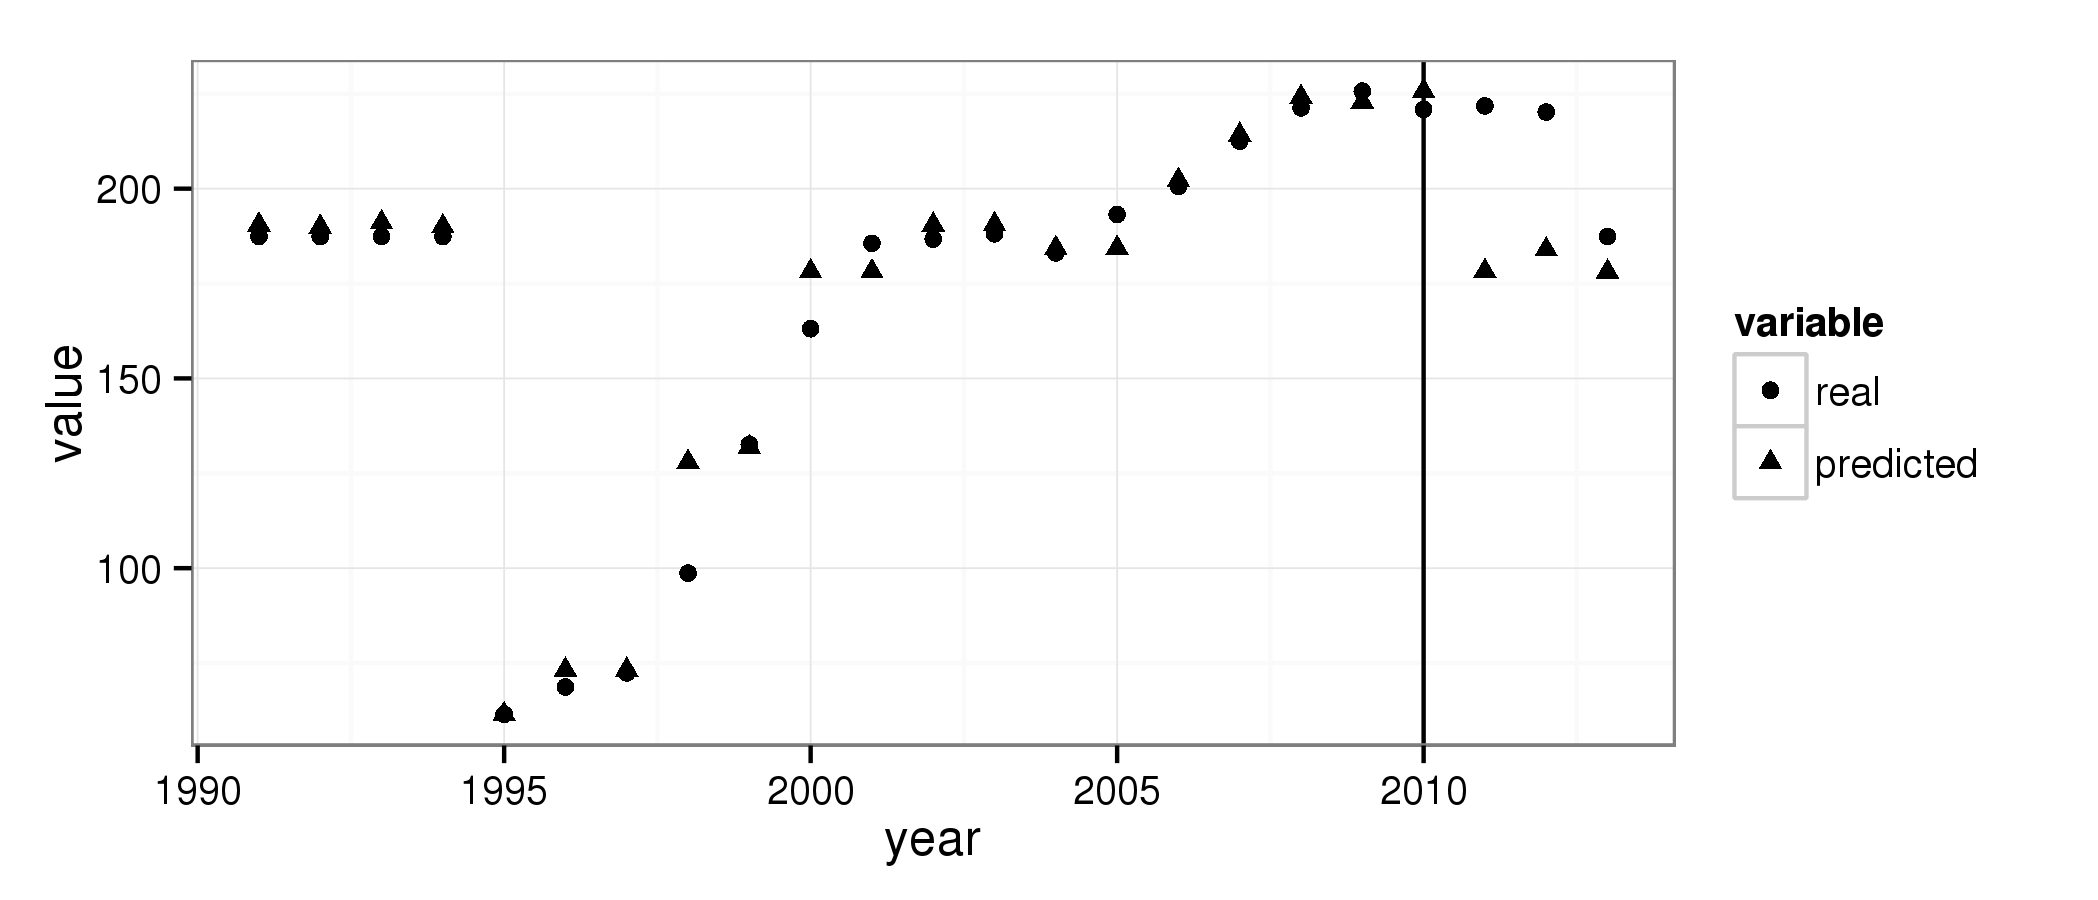
\includegraphics{images/m_plot1.png}
        \caption{Прогноз с набором показателей №1, горизонт 3 года.}		
        \label{figure:m_plot1}
    \end{center}
\end{figure}

\begin{figure}[bhtp]
    \begin{center}
        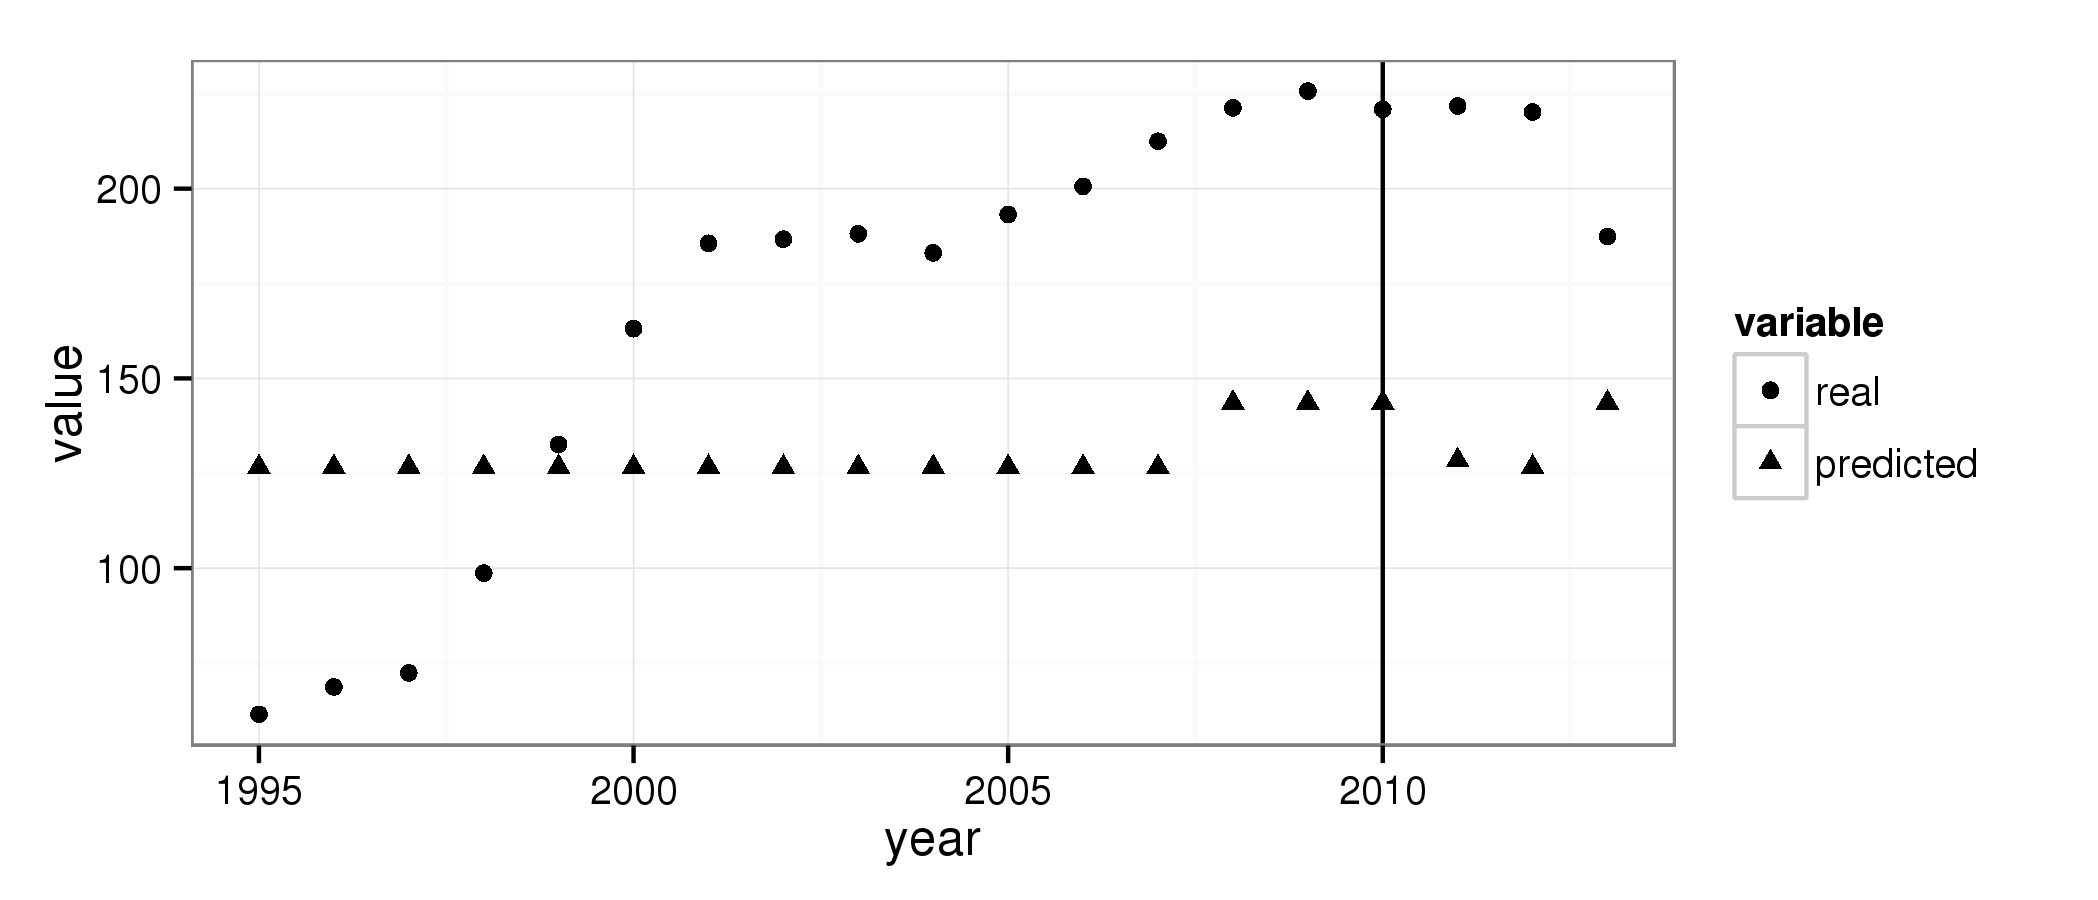
\includegraphics{images/m_plot2.png}
        \caption{Прогноз с набором показателей №2, горизонт 3 года.}		
        \label{figure:m_plot2}
    \end{center}
\end{figure}

\begin{figure}[bhtp]
    \begin{center}
        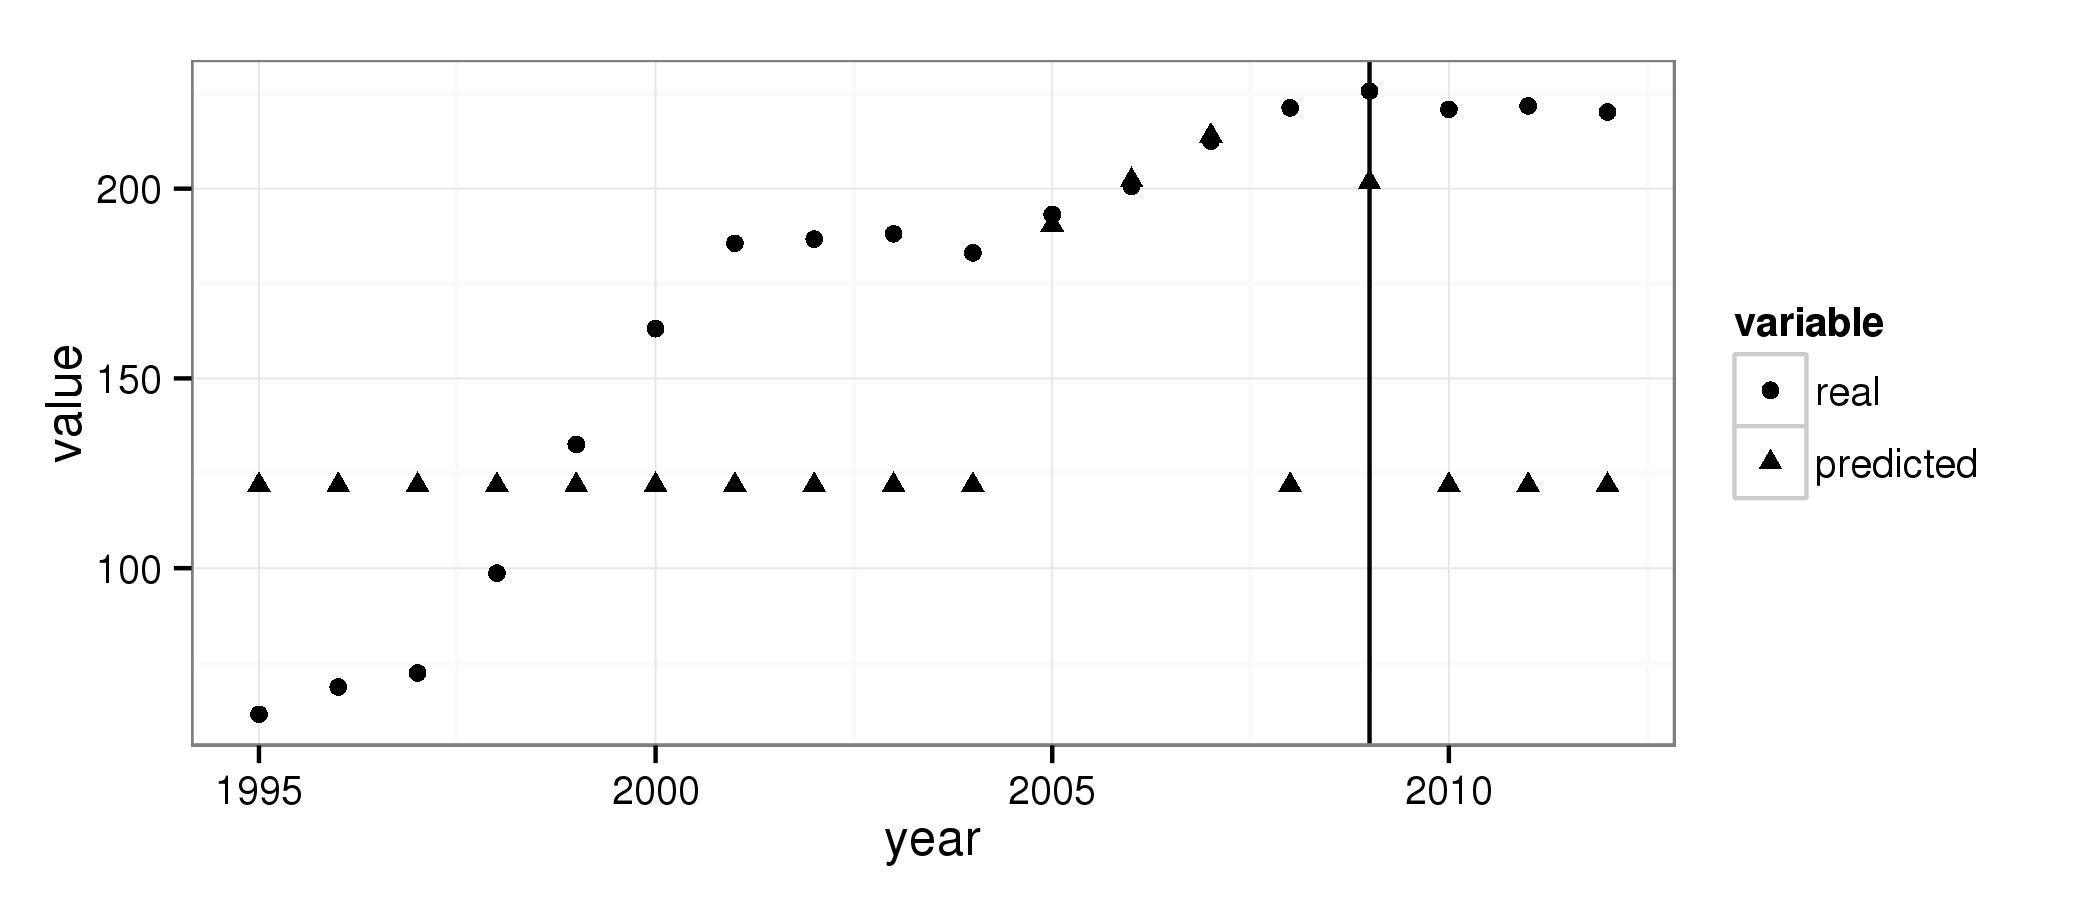
\includegraphics{images/m_plot3.png}
        \caption{Прогноз с набором показателей №3, горизонт 3 года.}		
        \label{figure:m_plot3}
    \end{center}
\end{figure}

С точки зрения точности прогноза, при использовании набора показателей №1
наблюдается существенное улучшение относительно одномерного варианта.  Однако,
требуемый уровень точности на данный момент не достигнут.

Низкие оценки точности прогноза при использовании наборов показателей №2 и №3
объясняются, по мнению автора, неполнотой исходных данных, которая выражается в
наличии пропущенных значений в независимых переменных, требующих их
экстраполяции (в нашем случае для заполнения пропусков использовалась функция
медианы), что заведомо снижает количество доступной для модели информации, и
искажает характеристики случайных величин, тем самым нарушая механизмы
прогнозирования.

\newpage
\section{Формальное описание модели}
Предлагаемая модель прогнозирования численности наркозависимых на основе
нечеткой логики состоит из ряда последовательных аналитических шагов:
\begin{enumerate}
    \item Определение исходных данных;
    \item Заполнение пропусков в исходных данных (imputation);
    \item Выбор горизонта прогнозирования;
    \item Обучение модели с помощью алгоритма нечетко-логического вывода;
    \item Получение результатов модели (численных значений временных рядов,
        оценок ошибки прогнозирования, связей между переменными и др.);
    \item Интерпретация результатов модели 
\end{enumerate}
Остановимся на некоторых из данных шагов подробнее. 

\textit{Определение исходных данных.}. Модель относится к категории моделей с
множеством входных переменных и одной выходной переменной (MISO). Это означает,
что прежде всего определиться с целевой переменной, прогнозирование которой и
будет осуществляться. В нашем случае, это показатель "Состоит на учете больных с
диагнозом <<наркомания>>, на 100 тыс. населения", полученный из Информационной
системы информационно-аналитического обеспечения органов государственной власти
Санкт-Петербурга. Однако, в <<сыром>> виде использовать показатели оценки
наркоситуации не эффективно, т.к. ситуация, наблюдаемая органами государственной
статистики и объективная ситуация, как правило, расходятся на несколько порядков
ввиду нелегальной природы самого феномена наркотизма, наркорынков и пр. Для
объективной оценки феномена наркотизации вводится понятие коэффициента
латентности \cite{Zakharov2012}, определяемого как отношение фактического значения исследуемой
величины (в наешм случае --- числа наркозависимых) к наблюдаемому значению.
Оценка коэффициента латентности выходит за рамки данного исследования, добавим
лишь, что как правило латентный анализ используется  в сопряжении с установкой и
анализом пороговых уровней, позволяющих судить о степени кризисности ситуации в
зависимости от принадлежности тех или иных целевых величин соответствующим
уровням. Кроме того, для приведения модели к стандартизированному виду,
возможности её сопоставления с аналогами из Банка моделей и для внедрения
элементов вероятностного моделирования целесообразно переводить абсолютные
значения исследуемой величины в вероятность или долю (в нашем случае ---
вероятность заболевания наркозависимостью для отдельно взятого человека). Таким
образом, общая формула манипуляций, производимых с исследумой переменной до
непосредственно процесса прогнозирования выглядит следующим образом:

\begin{equation}
    p_{addiction} = \frac{\rho_{drug}}{\rho_{population}}\cdot k
\end{equation}

Где \(p_{addiction}\) --- вероятность заболевания наркозависимостью для отдельно
взятого человека, \(\rho_{drug}\) --- численность наркозависимых по данным
официальной статистики, \(\rho_{population}\) --- численность населения города
Санкт-Петербурга, \(k\) --- коэффициент латентности.

Далее необходимо определиться с составом входных переменных. Модель базируется
на предположении о существовании явной или неявной связи между входными
переменными и выходной переменной. Социальные процессы не связаны такими же
жесткими законами, как физические процессы, но можно предложить методы подбора
входных переменных, способных обеспечить максимальную точность прогнозирования.
К таким методам можно отнести: использование экспертного знания (исследований,
опросов, метода коллегиальной оценки, гипотез и др.), обращение к аппарату
теоретико-методологических основ в исследуемой предметной области, проведение
корреляционного анализа. Помимо этого, модель, в силу своей универсальности,
прдполагает возможность проведения сценарного анализа для учета влияния не
только наркоспецифических, но и общеэкономических и социальных факторов для
обнаружения и потенциального устранения непредвиденного влияния изменений в
какой-либо из сфер жизнедеятельности города на состояние наркоситуации.

\textit{Заполнение пропусков в исходных данных.} Основой моделирования
наркоситуации являются данные государственной статистики.  Однако, на практике,
данные статистических служб имеют свои особенности и ограничения, которые
необходимо учитывать при моделировании. К ним относятся: изменение год от года
методик сбора данных, наличие переходных периодов, когда данные не собираются,
разная частота и периодичность сбора данных в зависимости от конкретных
показателей. Это приводит к неоднородности исходных данных, необходимости их
приведения к нормализованному виду для дальнейшего анализа.  Необоходимость
решения данной задачи обусловлена ещё и тем, что зачастую требуется использовать
максимально длинный временной ряд ввиду того, что точность моделей на основе
алгоритмов машинного обучения прямо пропорциональна объему доступной для
обучения информации. И если взять за основу максимально длинный временной ряд,
неизбежно возникают пропуски в случаях его совместного использования с
сопутствующими временными рядами.  Для решения этой задачи используются методы
т.н. <<imputation>> или заполнения пропусков в данных. К таким методам относятся
функции агрегирования (например, месячные, годовые средние, медианы и т.п.),
аппроксимирования (интерполяции, сплайны и др.), метод LOCF (<<последнее
наблюдаемое значение переносится вперёд>>), фильтры (например, сезонный фильтр
Калмана), наконец, ручное заполнение пропущенных значений и обрезание
пропущенных значений в конце и начале временного ряда. Выбор конкретного метода
зависит от задач исследования, но в целом следует понимать, что заполнение
пропусков  может привести к искажениям в исходных данных.

\textit{Выбор горизонта прогнозирования.} Горизонт прогнозирования --- это
количество единиц времени в будущем, для которых требуется осуществить прогноз.
В анализе накроситуации применяются как среднесрочные прогнозы, так и
долгосрочные, в зависимости от актуальных задач.  Предлагаеая модель
ориентирована на краткосрочные и среднесрочные прогнозы ввиду ограниченности
исходных данных для построения более длинных предсказаний.

\textit{Обучение модели с помощью алгоритма нечетко-логического вывода.}
В качестве базового алгоритма обучения в работе используется  алгоритм
Ванга-Менделя, основанный на равномерном разбиении входного и выходного
пространств и построения отображения, учитывающего взаимное изменение уровней
переменных. Алгоритм подробнее описан в разделе 3.1.2 <<Методика проведения
эксперимента>>.

\textit{Получение результатов модели.} К результатам модели можно отнести ряд
аналитических продкутов. Это, прежде всего, численные значения временных рядов
на период, определённый установленным горизонтом прогнозирования,
соответствующие им оценки ошибки прогнозирования. Отельно следует затронуть
генерируемую моделью базу нечетких правил. Нечеткие правила типа <<ЕСЛИ,ТО>>
описывают связи между переменными, в зависимости от их уровней, описываемых
лингвистическими переменными. Например, правило может звучать так: Если уровень
безработицы высок, то численность наркозависимых выше среднего. При этом понятия
<<высоко>> и <<выше среднего>> могут быть уточнены путем сопоставления отдельных
термов лингвистических переменных конкретным значениям функций принадлежности.

\textit{Интерпретация резултьтатов модели.} Учитывая, что основных аналитических
продуктов модели два, каждый из них интерпретируется по-своему. Прогнозные
значения могут оцениваться как сами по себе, так и контексте определённых
пороговых уровней. В зависимости от попадания значений в те или иные уровни и от
общей направленности тренда можно говорить о степени кризисности наркоситуации и
планировать соответствующие контрмеры. База нечетких правил позволяет
исследовать связи между переменными, использую обнаруженные зависимости для
создания предложений о том, как можно повлиять на ситуацию для её наилучшего
развития.

\newpage
\section*{Выводы по главе 3}
\addcontentsline{toc}{section}{Выводы по главе 3}

Экспериментальная часть данного исследования была направлена на сравнение нечетко-логического и теоретико-множественного (теория нечетких временных рядов) подходов на примере авторегрессии по одной переменной. Согласно результатам эксперимента, нечетко-логический подход показал неудовлетворителньые резуьтаты на заданных данных. Приведены варианты разрешения этой трудности.

В части многомерного моделирования данное исследование было направлено на
сравнение точности прогнозной модели при использовании разных входных
индикаторов наркоситуации.  Согласно результатам эксперимента, наблюдается
значительное улучшение точности при условии достаточного объема и низкой
зашумленности исходных данных. 

Приоритетными направлениями дальнейшей деятельности являются:
\begin{itemize}
	\item Анализ предметной области <<Наркоситуация в Санкт-Петербурге>> с целью выделения релевантных показателей для прогнозирования.
	\item Использование API информационно-аналитической системы <<Антинар>> для упрощения доступа к данным государственной статистики.
	\item Создание графического интерфейса пользователя (предположительно с помощью библиотеки Shiny) с тем, чтобы обеспечить возможность использования моделей более широким кругом пользователей.
    \item Более тщательный и полный выбор показателей для прогнозирования. 
        (Возможно использование данных в разрезе по полу, возрасту; разбивка 
        временных рядов на месяца вместо годов и т.п.);
    \item Обеспечение стабильно-высокой точности прогноза;
    \item Интеграция модели прогнозирования в <<ИС ИАО>>.
\end{itemize}
	 

\chapter*{Заключение}
\addcontentsline{toc}{chapter}{Заключение}
Прогнозирование социально-экономических процессов в целом и наркоситуации в
частности --- один из наиболее важных инструментов для поддержки принятия
решений при управлении региональным развитием, который позволяет планировать
действия и ресурсы  в соответствии с гипотетическим состоянием социальной
системы в будущем.

Немаловажным обстоятельством является включенность системы
информационно-аналитической поддержки контроля за наркоситуацией в
общегосударственную стратегию антинаркотической политики, что требует строгой
подчиненности данной системы целям и задачам, выдвигаемым на данном этапе
реализации антинаркотической политики. Поэтому применяемые методы должны
максимально эффективно обеспечивать достижение целей мониторинга и анализа
наркоситуации.

Основные теоретические результаты работы носят следующий характер: 
\begin{itemize}
\item Изучены используемые в мировой практике антинаркотические политики;
\item Изучены методы и модели прогнозирования временных рядов;
\item Проведено сравнение моделей на предмет их эффективности в региональном
управлении;
\item Сформулированы требования к требуемой модели прогнозирования численности
наркозависимых на территории Санкт-Петербурга;
\item Спроектирован программный модуль прогнозирования для
информационно-аналитической системы.
\end{itemize}

В области практических результатов удалось достичь следующего:
\begin{itemize}
\item Модифицирована модель прогнозирования на основе нечеткой логики под нужды
анализа наркоситуации;
\item Разработан модуль прогнозирования для информационно-аналитической системы;
\item Разработаны рекомендации к применению новой модели и соответствующего
    программного инструмента;
\item Продемонстрированы характеристики интеллектуального анализа данных как
средства регионального управления.
\end{itemize}

В связи с тем, что с каждым годом наркоситуация сопровождается всё новыми
вызовами, одними из последних для примера можно назвать распространение
синтетических наркотиков, требуются ответы на эти вызовы. В том числе это
касается подсистемы информационно-аналитического обеспечения принятия решений.
Разработанная модель и сопутствующий  программный инструмент в силу своей
универсальности могут быть не только использованы для решения своей прямой
задачи --- прогнозирования численности наркозависимых, но и могут быть
адаптированы для других задач, в особенности имеющих отношение к сложным,
многосоставным связям между явлениями.

Разработанный инструмент, учитывая рекомендуемые условия его применения,  можно
рекомендовать к внедрению в качестве компонента информационно-аналитической
системы. Следует отметить обнаружившееся в ходе работы обстоятельство наличия у
интеллектуальных методов прогнозирования специфических аналитических продуктов,
удобных инструментов анализа которых пока что не обнаружено. В случае нечеткой
логики таким продуктом является база нечетких правил. Таким образом, можно
утверждать о необходимости развития области интеллектуального моделирования и
прогнозирования для наилучшего применения теоретических достижений на практике.

\newpage
\printbibliography[heading=bibintoc]

\end{document} % конец документа


